%%%%%%%%%%%%%%%%%%%%%%%%%%%%%%%%%%%%%%%%%%%%%%%
% Template baseado no exemplo da classe utftex
% Prof. César M. V. Benítez, Daniel Rossato
% DAELN, UTFPR-Curitiba (2020)
%%%%%%%%%%%%%%%%%%%%%%%%%%%%%%%%%%%%%%%%%%%%%%%


\documentclass[openright]{normas-utf-tex} %openright = o capitulo comeca sempre em paginas impares
%\documentclass[oneside]{normas-utf-tex} %oneside = para numero de paginas menor que 100 (apenas frente da folha) 

% force A4 paper format
\special{papersize=210mm,297mm}

\usepackage[alf,abnt-emphasize=bf,bibjustif,recuo=0cm, abnt-etal-cite=2, abnt-etal-list=99]{abntcite} %configuracao correta das referencias bibliograficas.

\usepackage[portuguese, ruled, linesnumbered]{algorithm2e}%pacotedealgoritmoemportugues

\usepackage[table]{xcolor}
\usepackage[brazil]{babel} % pacote portugues brasileiro
\usepackage[utf8]{inputenc} % pacote para acentuacao direta
\usepackage{amsmath,amsfonts,amssymb} % pacote matematico
\usepackage{graphicx} % pacote grafico
\usepackage{times} % fonte times
\usepackage[final]{pdfpages} % adicao da ata
\usepackage[version=3]{mhchem}%adição de pacote para quimica
% \usepackage{longtable}% redimensionar automaticamente tabelas
\usepackage{subfig}
\usepackage{relsize}
\usepackage[paper=portrait,pagesize]{typearea}
\usepackage{pdflscape}
\usepackage{url}

% minted
\usepackage{minted}

% adicionando bordas ao código em 'minted'
\usepackage{tcolorbox}
\usepackage{etoolbox}
\BeforeBeginEnvironment{minted}{\begin{tcolorbox}}%
\AfterEndEnvironment{minted}{\end{tcolorbox}}%

% numeração de fórmulas
\usepackage{amsmath}
%\numberwithin{equation}{section}

%\usepackage{hyperref}% link das res
\newcommand\tab[1][1cm]{\hspace*{#1}}

%Podem utilizar GEOMETRY{...} para realizar pequenos ajustes das margens. Onde, left=esquerda, right=direita, top=superior, bottom=inferior. P.ex.:
%\geometry{left=3.0cm,right=1.5cm,top=4cm,bottom=1cm} 
\usepackage{amsthm}
\newtheorem{mydef}{Definicão}

%\usepackage{balance} 

% ---------- Preambulo ----------
\instituicao{ UNIVERSIDADE TECNOLÓGICA FEDERAL DO PARANÁ (UTFPR)} % nome da instituicao
\programa{Projeto REA} % nome do programa
\area{Engenharia Mecânica} 
\documento{PROGRAMA DE APOIO AO DESENVOLVIMENTO DE RECURSOS EDUCACIONAIS ABERTOS NA GRADUAÇÃO DA UTFPR (ÁREAS TRANSVERSAIS)}
\nivel{Graduação em Engenharia Mecânica} 
\titulacao{Graduação em Engenharia Mecânica}

\titulo{RECURSOS DE INTERACAO EDUCACIONAL DIGITAL APLICADOS A FISICA, QUIMICA, A MATEMATICA E AS ENGENHARIAS USANDO O SCILAB E O PYTHON} % titulo do trabalho em portugues

% \title{\MakeUppercase{Título em Inglês}} % titulo do trabalho em ingles

\autor{ Igor De Paula Nascimento Lima \\ 
	Joe Michael Hideyuki Furuya Takahassi \protect} % autor do trabalho

%\cita{aluno1} % sobrenome (maiusculas), nome do autor do trabalho


\palavraschave{palavra chave}  % palavras-chave do trabalho
\keywords{keywords} % palavras-chave do trabalho em ingles

\comentario{Apostila elaborada para o projeto de Recursos Educacionais Abertos descritos no edital 26/2021 e ofertada pela UTFPR, apresentado aos avaliadores da banca como requisito para a conclusão do projeto.} 

\orientador{Prof. Dr. Antônio Carlos Amaro de Faria Júnior \protect} % nome do orientador do trabalho

\local{Curitiba} % cidade
\data{\the\year} % ano automatico

% desativa hifenizacao mantendo o texto justificado.
% thanks to Emilio C. G. Wille
\tolerance=1
\emergencystretch=\maxdimen
\hyphenpenalty=10000
\hbadness=10000
\sloppy

%---------- Inicio do Documento ----------
\begin{document}

\capa % geracao automatica da capa
\folhaderosto % geracao automatica da folha de rosto


% % dedicatoria (opcional)
% \begin{dedicatoria}
% Texto da dedicat\'oria. 
%\end{dedicatoria}

% % agradecimentos (opcional)
%\begin{agradecimentos}
% Texto dos agradecimentos.
%\end{agradecimentos}

% % epigrafe (opcional)
% \begin{epigrafe}
% Texto da ep\'igrafe.
% \end{epigrafe}

%resumo
%\begin{resumo}

% \end{resumo}

%abstract
% \begin{abstract}

% \end{abstract}

% listas (opcionais, mas recomenda-se a partir de 5 elementos)
\listadefiguras % geracao automatica da lista de figuras
\listadetabelas % geracao automatica da lista de tabelas
% \listadequadros % adivinhe :)
% \listadesiglas % geracao automatica da lista de siglas
% \listadesimbolos % geracao automatica da lista de simbolos

% sumario
\sumario % geracao automatica do sumario


%---------- Inicio do Texto ----------
% recomenda-se a escrita de cada capitulo em um arquivo texto separado (exemplo: intro.tex, fund.tex, exper.tex, concl.tex, etc.) e a posterior inclusao dos mesmos no mestre do documento utilizando o comando \input{}, da seguinte forma:
%\input{intro.tex}
%\input{fund.tex}
%\input{exper.tex}
%\input{concl.tex}

% Colocar aqui o numero da página inicial!!! (Obs.: conta a partir da folha de rosto)
\setcounter{page}{12}

\chapter{Introdução}

\section{Motivação} %qual o problema?
Esse material foi elaborado para o projeto "Recursos de Interação Educacional Digital Aplicados à Física, Química, à Matemática e às Engenharias usando o Scilab e o Python", ofertado pela UTFPR e pertencente ao Edital 26/2021. Para cada exemplo, foi exibido os respectivos códigos fontes assim como foi escrito uma explicação dos principais conceitos relacionados àquele tema. 

\section{Objetivos}
O objetivo do projeto é auxiliar o estudante no aprendizado de conceitos importantes tanto no campo da Física, Química, Matemática e Engenharias, através da elaboração de exemplos práticos no ambiente Jupyter Lab. Para isso, foi consultado referências bibliográficas para a elaboração da fundamentação teórica assim como foi utilizado algumas bibliotecas específicas do Python pertinentes para cada exemplo em questão.



%\subsection{Objetivo geral} 




%\subsection{Objetivos específicos} 
%\label{sec:objespecif}

   %Introducao
\chapter{Exemplos}

Nesta seção serão apresentados os exemplos práticos escolhidos para o projeto. 

\section{Exemplo de análise de tecnologia - Comunicação sem Fio}
\label{sec:exemplo}
Como mostrado na Seção \ref{sec:objespecif}, o projeto proposto necessita de um módulo de comunicação sem fio para interagir com o aplicativo no celular do usuário. Foram analisadas as tecnologias Wi-Fi e Bluetooth, visto que estas estão presentes em praticamente todos os \textit{smartphones} modernos.

\subsection{Wi-Fi}
\label{sec:wifi}

A tecnologia Wi-Fi é tecnologia de rede sem fio criada em 1998 pela Wi-Fi Alliance, baseada no padrão IEEE 802.11. Ela é hoje a tecnologia mais comum para conexão sem fio de dispositivos à internet em dispositivos pessoais \cite{WiFi2020}. Um dos módulos mais comuns para aplicações de \sigla{IoT}{Internet of Things} (Internet das Coisas) é o ESP8266 \cite{datasheet8266}, que tem baixo custo e fácil disponibilidade de compra. Este módulo é mostrado na Figura \ref{fig:esp8266}.

\begin{figure}[!htb]
	\centering
	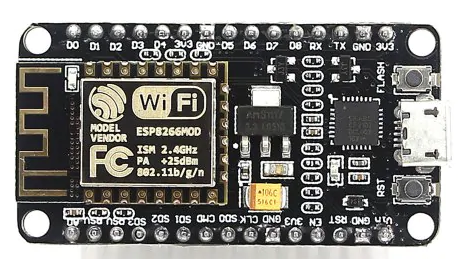
\includegraphics[width=0.4\textwidth]{./esp8266.png} 
	\caption{Foto do módulo Wi-Fi ESP8266.}
	\label{fig:esp8266}
\end{figure}

\subsection{Bluetooth}
\label{sec:bt}
A tecnologia Bluetooth foi criada em 1989, com o objetivo de substituir o protocolo RS-232 na comunicação de curta distância entre objetos fixos (citar referência). O módulo mais comum para IoT é o HC-05, mostrado na Figura \ref{fig:hc05}.

\begin{figure}[!htb]
	\centering
	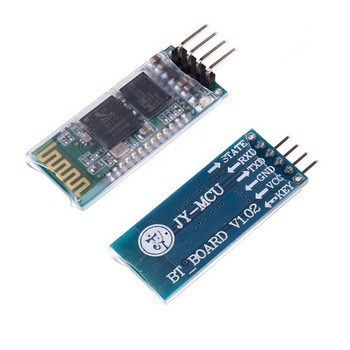
\includegraphics[width=0.4\textwidth]{./hc05.jpg} 
	\caption{Foto do módulo Bluetooth HC-05.}
	\label{fig:hc05}
\end{figure}

\subsection{Comparativo entre tecnologias de comunicação sem fio}
Na Tabela \ref{tab:semfio} são comparadas as principais características dos módulos ESP8266 e HC-05. Esta tabela foi criada com o auxílio do site \url{www.tablesgenerator.com}.

\begin{table}[!htb]
\centering
\begin{tabular}{l|l|l}
    ~       & ESP8266   & HC-05      \\
    \hline
    Alcance & 50m       & 10m        \\
    \hline
    Consumo & 170mA     & 40mA       \\
    \hline
    Preço   & R\$ 22,90 & R\$ 25,90  \\
    \hline
\end{tabular}
\caption{Comparativo entre módulos ESP8266 e HC-05}
\label{tab:semfio}
\end{table}

O módulo ESP8266 tem maior alcance e menor custo que o HC-05, como pode ser visto na Tabela \ref{tab:semfio}. Porém, como o projeto proposto será alimentado por bateria, é essencial diminuir o consumo de corrente do sistema. Por isso, foi escolhido o módulo HC-05. Além disso, o desenvolvimento de aplicações com comunicação Bluetooth já é dominado pela equipe, reduzindo a dificuldade da implementação.



   %Fundamentacao teorica
\chapter{Metodologia}

\section{Visão geral}


* Obs.: nao esqueça de apresentar o diagrama de blocos do sistema. 


\section{Projeto mecânico}


\section{Projeto de \textit{hardware}}


* Obs.: nao esqueça de apresentar o diagrama de blocos do hardware. 


\section{Projeto de \textit{software}}



* Obs.: nao esqueça de apresentar os diagramas de estados (statecharts) do 
software.


\section{Integração}









   %Metodologia
\chapter{Experimentos e resultados}

% testes, integração, etc.   %Experimentos e resultados
\section{Distribuição Gaussiana}

\subsection{O que é a Distribuição Gaussiana?}
A \textbf{distribuição Gaussiana} ou \textbf{distribuição normal} é uma das distribuições mais importantes em razão da sua enorme presença nos mais variados campos do conhecimento. Se trata de uma curva de distribuição simétrica em torno do seu ponto médio. Ela possui a peculiaridade de ter a média, mediana e moda dos dados com o mesmo valor.

\subsection{Variável aleatória]}
\textbf{Variável aleatória} é um valor retirado de uma distribuição estatística e que não possui um valor fixo. O seu valor depende de fatores aleatórios. Ex: o resultado do lançamento de um dado pode dar qualquer número entre 1 e 6.

Uma variável aleatória que pode assumir apenas um número finito ou uma sequência infinita enumerável de valores é considerada \textbf{discreta}. Aquele que pode assumir qualquer valor no intervalo dos números reais é considerado \textbf{contínuo}. 

Uma \textbf{variável aleatória contínua} é uma variável aleatória que pode tomar qualquer valor numérico em um determinado intervalo ou coleção de intervalos (geralmente do conjunto dos números reais). Ex: uma variável aleatória que mede o tempo que leva para algo ser feito é contínua, pois ela pode assumir infinitos valores.

Como existe um número infinito de valores em qualquer intervalo, não faz sentido falar sobre a probabilidade da variável aleatória assumir um valor específico. Em vez disso, é considerada a probabilidade de uma variável aleatória contínua estar dentro de um determinado intervalo. É a chamada \textbf{Função Densidade de Probabilidade}.

\subsection{Função Densidade de Probabilidade}

É a função $f(x)$  de uma variável aleatória contínua cuja integral em um intervalo dá a probabilidade de que o valor da variável esteja dentro desse mesmo intervalo. Ou seja, \textbf{densidade de probabilidade} não é probabilidade. Somente quando a função for integrada entre dois limites é que ela produzirá uma probabilidade, sendo equivalente à área sob a curva da função densidade de probabilidade entre esses dois limites:

\[\large \int_{a}^{b} f(x)dx = P(a\leq x\leq b)\]

As funções densidade de probabilidade devem sempre obedecer à esses 2 requisitos:
\begin{itemize}
\item $f(x)$ deve ser não negativo para cada valor da variável aleatória: $f(x) > 0$
\item A área total sob a curva de probabilidade vale sempre 1: $\int_{-\infty }^{\infty} f(x)dx = 1$
\end{itemize}

A forma da função de densidade de probabilidade em todo o seu domínio é chamada de \textbf{distribuição de probabilidade}. A distribuição de probabilidade mais importante é a chamada \textbf{distribuição normal}, também chamado de \textbf{curva em forma de sino} devido à sua forma característica.

\subsection{Distribuição Normal ou Gassiana}

A distribuição normal é a distribuição de probabilidade mais importante no estudo da estatística devido à sua presença em muitos fenômenos naturais, por exemplo: a altura das pessoas, pressão arterial, erro de medição e pontuações de QI seguem a distribuição normal.

Como já foi dito, a probabilidade de uma observação assumir um valor entre dois pontos quaisquer é igual à área sob a curva da densidade de probabilidade compreendida entre esses dois pontos. No caso de uma curva de distribuição normal teórica, a regra é: 

\begin{itemize} 

\item $68,26\%$ da população ou amostra está dentro de uma região que varia de $\mu \pm \sigma$ 
\item $95,44\%$ da população ou amostra está dentro de uma região que varia de $\mu \pm 2\sigma$
\item $99,72\%$ da população ou amostra está dentro de uma região que varia de $\mu \pm 3\sigma$
\item $99,99\%$ da população ou amostra está dentro de uma região que varia de $\mu \pm 4\sigma$ 

\end{itemize}

\begin{figure}[H]
	\centering
	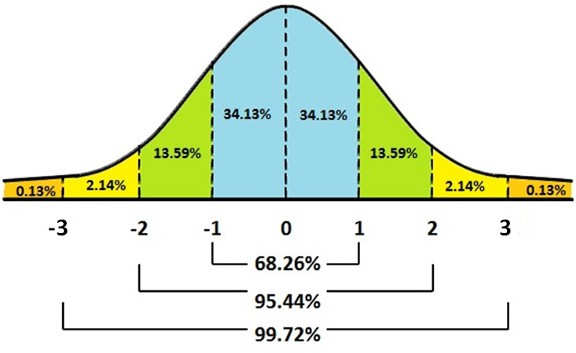
\includegraphics[width=1\textwidth]{./Imagens/Distribuição Normal/GA1.png} 
	\caption{Distribuição normal}
	\label{fig:GA1}
\end{figure}

\subsection{Densidade para a distribuição normal}
Uma variável aleatória contínua X tem distribuição normal se sua função densidade de probabilidade for dada por:

\[ \large p(x) = \frac{1}{\sigma \sqrt{2 \pi  }}e^{-\frac{1}{2} (\frac{x-\mu}{\sigma})^2} \]

Onde $\sigma$ é o \textbf{desvio padrão} da distribuição e $\mu$ é a \textbf{média}.

\subsection{Desvio padrão}

Comumente representado pelo símbolo $\sigma$, é uma medida de dispersão em torno da média populacional ou amostral de uma variável aleatória. Quanto maior o seu valor maior a ampla de valores na qual os dados estão espalhados. Um baixo desvio padrão indica que os pontos dos dados tendem a estar próximos da média.

\subsection{Fórmula para o desvio padrão}

O desvio padrão populacional ou amostral é a raiz quadrada da variância populacional ou amostral correspondente. 

\begin{itemize}

\item Quando o conjunto de dados é a população:

\[ \large \sigma = \sqrt{\frac{1}{N}\sum_{i=1}^{N}(x_{i}-\mu )^2} \]

\item Quando o conjunto de dados é uma amostra:

\[ \large \sigma = \sqrt{\frac{1}{N-1}\sum_{i=1}^{N}(x_{i}-\mu )^2} \]

\end{itemize}

\subsection{Distribuição Normal no Python}

Vamos traçar a curva de uma \textbf{distribuição normal padronizada}, que é uma curva normal de média $\mu = 0$ e desvio padrão $\sigma = 1$.

\begin{minted}{python}
	
from scipy.stats import norm
import matplotlib.pyplot as plt
import numpy as np 

fig, ax = plt.subplots(figsize = (8,5))

# definindo o domínio
dom = np.linspace(-2,2,1000)

plt.plot(dom, norm.pdf(dom, loc = 0 , scale = 1))
plt.title("Distribuição Normal Padronizada")
plt.xlabel("Valor")
plt.ylabel("Densidade")
ax.grid(True)
plt.show()

\end{minted}

\begin{figure}[H]
	\centering
	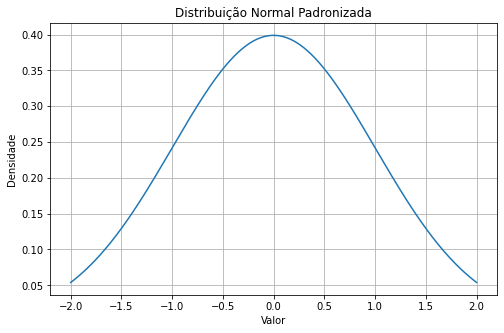
\includegraphics[width=1\textwidth]{./Imagens/Distribuição Normal/GA2.png} 
	\caption{Curva normal}
	\label{fig:GA2}
\end{figure}

Podemos alterar a forma da curva em sino alterando a média e o seu desvio padrão. Alterar a média deslocará a curva em direção a esse valor, isso significa que podemos alterar a posição da curva alterando o valor médio sem afetar a forma da curva.

\begin{minted}{python}
	
fig, ax = plt.subplots(figsize = (8,5))

x = np.linspace(-10,15,100)

medias = [0.0, 2.0, 5.0, 10.0]

for medias in medias:
ax.plot(x, norm.pdf(x,loc=medias), label=f"Médias: {medias}")

ax.set_xlabel('x')
ax.set_ylabel('pdf(x)')
ax.set_title('Distribuição Normal')
ax.legend(loc='best', frameon=True)
ax.set_ylim(0,0.45)
ax.grid(True)
	
\end{minted}

\begin{figure}[H]
	\centering
	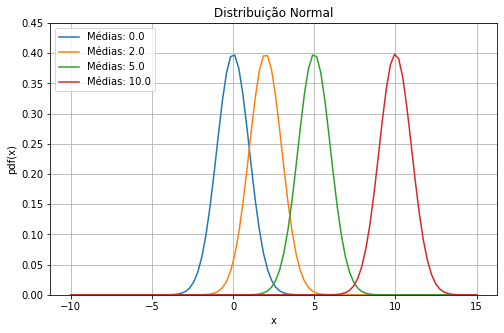
\includegraphics[width=1\textwidth]{./Imagens/Distribuição Normal/GA3.png} 
	\caption{Alterando a média}
	\label{fig:GA3}
\end{figure}

A forma da curva pode ser controlada pelo valor do desvio padrão. Um desvio padrão menor resultará em uma curva estreitamente limitada, enquanto um valor alto resultará em uma curva mais espalhada. 

\begin{minted}{python}
	
fig, ax = plt.subplots(figsize = (8,5))

x = np.linspace(-10,10,100)

stdvs = [1.0, 2.0, 3.0, 4.0]

for s in stdvs:
ax.plot(x, norm.pdf(x, scale=s), label=f'desvio padrão = {s}')

ax.set_xlabel('x')
ax.set_ylabel('pdf(x)')
ax.set_title('Distribuição Normal')
ax.legend(loc='best', frameon=True)
ax.set_ylim(0,0.45)
ax.grid(True)
	
\end{minted}

\begin{figure}[H]
	\centering
	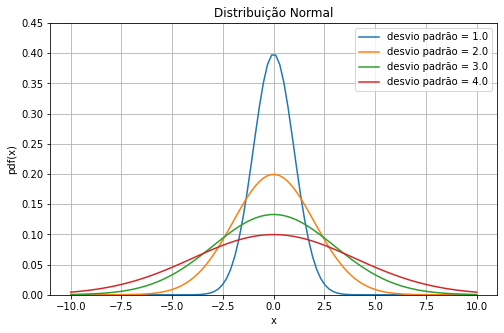
\includegraphics[width=1\textwidth]{./Imagens/Distribuição Normal/GA4.png} 
	\caption{Alterando o desvio padrão}
	\label{fig:GA4}
\end{figure}

\subsection{Função distribuição acumulada}

É a função $F(x)$ que indica a probabilidade de um determinado valor de uma variável aleatória X ser menor ou igual à x. Em termos matemáticos:

\[\large F(x) = P(X \leq x) = \int_{-\infty }^{x}f(x_{i})dx\]

\subsubsection{Calculando a probabilidade de ocorrência de dados específicos}

Vamos utilizar o conceito de função distribuição acumulada (CDF) e calcular a probabilidade de um valor estar abaixo de -1 ao escolhermos um valor aleatório da distribuição. Essa probabilidade será a área da região apresentada abaixo e terá um valor de aproximadamente $15,87\%$.

\begin{figure}[H]
	\centering
	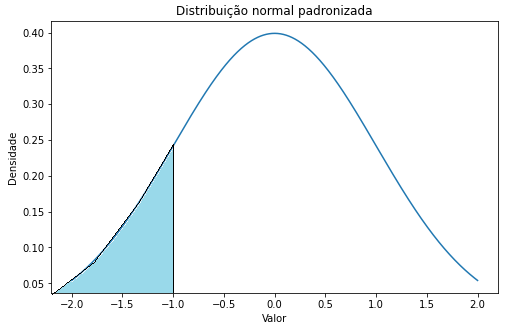
\includegraphics[width=1\textwidth]{./Imagens/Distribuição Normal/GA5.png} 
	\caption{Abaixo de -1}
	\label{fig:GA5}
\end{figure}

\begin{minted}{python}
prob = norm(loc = 0 , scale = 1).cdf(-1)
print(f"Probabilidade: {prob*100:.2f}%")
# Probabilidade: 15.87%
\end{minted}

Para calcular a probabilidade do valor estar entre uma região específica (entre 2 e 1 por exemplo):

\begin{figure}[H]
	\centering
	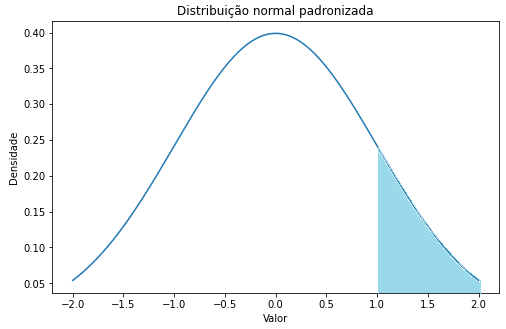
\includegraphics[width=1\textwidth]{./Imagens/Distribuição Normal/GA6.png} 
	\caption{Entre 1 e 2}
	\label{fig:GA6}
\end{figure}

\begin{minted}{python}
cdf_limite_superior = norm(loc = 0 , scale = 1).cdf(2)
cdf_limite_inferior = norm(loc = 0 , scale = 1).cdf(1)

prob = cdf_limite_superior - cdf_limite_inferior
print(f"Probabilidade: {prob*100:.2f}%")
# Probabilidade: 13.59%
\end{minted}

Para calcular a probabilidade do valor ser maior que x (0.5 por exemplo): 

\begin{figure}[H]
	\centering
	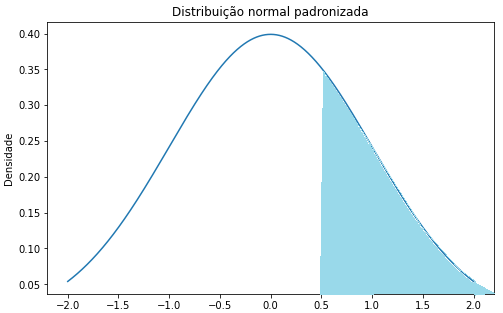
\includegraphics[width=1\textwidth]{./Imagens/Distribuição Normal/GA7.png} 
	\caption{Maior que 0.5}
	\label{fig:GA7}
\end{figure}

\begin{minted}{python}
prob = 1 - norm(loc = 0 , scale = 1).cdf(0.5)
print(f"Probabilidade: {prob*100:.2f}%")
# Probabilidade: 30.85%
\end{minted}

\subsection{Aplicações da Distribuição Normal}
\begin{itemize}
\item O matemático francês Abraham de Moivre, em seu Doctrine of Chances (1718), primeiro observou que as probabilidades associadas a variáveis aleatórias geradas discretamente (como as obtidas jogando uma moeda ou jogando um dado) podem ser aproximadas pela área sob o gráfico de uma função exponencial. Este resultado foi estendido e generalizado pelo cientista francês Pierre-Simon Laplace.
\item Em 1860, Maxwell supôes que a velocidade das colisões das partículas obedecem a distribuição normal.
\item Pode ser utilizado na análise da resistência dos materiais, onde os dados coletados podem ser generalizados para uma distribuição normal de forma a facilitar as simulações computacionais e torná-los mais práticos. 
\item Em projetos de engenharia no campo da ergonomia.
\end{itemize}   %Cronograma e custos do projeto
\section{Integral de Riemann}

\subsection{Conceito de Integral}

Em cálculo, o conceito de integral se refere à soma infinitesimal de regiões para se obter o valor total de uma região contínua. Ela pode ser considerada uma área ou a generalização de uma área e, juntamente com a derivada, constitui os conceitos fundamentais do Cálculo.

O exemplo mais simples de integral é a \textbf{Integral de Riemann}. Considerando uma função contínua $f(x)$ num intervalo $[a,b]$ tal que $f(x) \geq 0$  para todo $x \; \epsilon \; [a,b]$, a sua curva plotada no sistema cartesiano fica:

\begin{figure}[H]
	\centering
	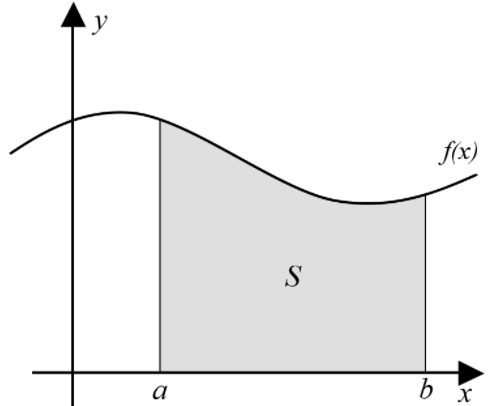
\includegraphics[width=0.8\textwidth]{./Imagens/Integral de Riemann/RI1.png} 
	\caption{Área sob a curva}
	\label{fig:RI1}
\end{figure}

\subsection{Integral de Riemann}

O valor total da área sob a curva da função $f(x)$ pode ser obtido dividindo essa área em diversos retângulos menores com extremidades nos pontos $[x_{0}, x_{1}, x_{2}, x_{3}, ..., x_{n}]$. A fórmula para a Integral de Rieman basicamente diz que a área da região compreendida entre o eixo horizontal e o gráfico da função $f(x)$, para x percorrendo o intervalo $[a,b]$, é igual ao limite da soma das áreas dos $n$ retângulos, quando o número desses retângulos tende a infinito.

\begin{figure}[H]
	\centering
	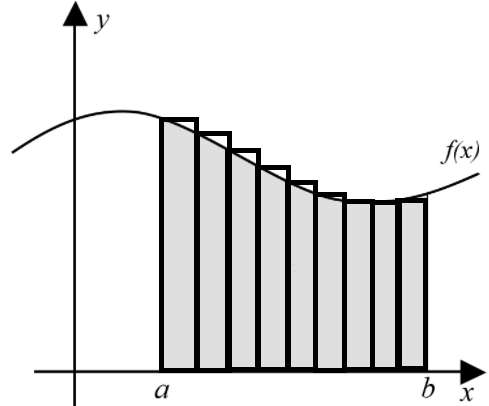
\includegraphics[width=0.8\textwidth]{./Imagens/Integral de Riemann/RI2.png} 
	\caption{Divisão da área}
	\label{fig:RI2}
\end{figure}

\subsubsection{Fórmula}

A Integral de Riemann da função $f(x)$ em relação a $x$ de $a$ para $b$ é: 

\begin{equation}
\large \int_{a}^{b}f(x) \; dx = \lim_{n \rightarrow \infty}\sum_{i=1}^{n} \frac{b-a}{n}f(x_{i-1})
\tag{5.1}
\end{equation}

A integral corresponde à "área com sinal", isto é, a área acima do eixo $x$ é positiva e a área abaixo do eixo $x$ é negativa.

Quando ela possui 2 limites, a integral é do tipo \textbf{definida}. Integral sem limite é denominada \textbf{indefinida}.

\subsection{Função primitiva/integral indefinida/antiderivada}

A \textbf{função primitiva/integral indefinida/antiderivada} de uma função $f$ é uma função diferenciável $F$ cuja derivada é igual à função original $f$. Isso pode ser representado simbolicamente por $F' = f$.

O processo de calcular funções primitivas (ou integrais indefinidas) de funções é oposto ao da diferenciação de funções, cujo objetivo é obter a derivada. Funções primitivas geralmente são representados por letras maiúsculas e estão relacionadas às integrais definidas pelo \textbf{Teorema Fundamental do Cálculo}.

Exemplo: 

A função $F(x) = \frac{x^3}{3}$ é a função primitiva de $f(x) = x^2$ uma vez que a derivada de $F(x) = \frac{x^3}{3}$ é $x^2$. Uma vez que a derivada de uma constante é zero, $x^2$ possuirá infinitas funções primitivas da forma $F(x) = \frac{x^3}{3} + C$ onde $C$ é denominada constante de integração.

\subsection{Teorema Fundamental do Cálculo}

O \textbf{Teorema Fundamental do Cálculo} diz que se $f(x)$ é uma função contínua em $[a,b]$, a sua integral definida nesse intervalo é a diferença entre as suas funções primitivas $F(x)$ nas extremidades desse intervalo:

\begin{equation}
\large \int_{b}^{a}f(x)\:dx = F(b) - F(a) = F(x)|^{b}_{a}
\tag{5.2}
\end{equation}

\subsection{Integral de Riemann utilizando scipy do Python}
Vamos utilizar a função \textbf{quad} da biblioteca Scipy para realizar a integração da função abaixo:

\begin{equation}
\large \int_{0}^{4}x^2dx
\tag{5.3}
\end{equation}

Para isso, vamos utilizar a função \textbf{lambda} do Python, que permite a criação de funções com número qualquer de argumentos:

\begin{minted}{python}
	x2 = lambda x: x**2
	print(x2)
	print(type(x2))
\end{minted}

Após isso, usamos a a função \textbf{integrate} da biblioteca \textbf{scipy} para realizar a integração.

O valor retornado pela função é uma tupla, onde o primeiro elemento é o valor estimado da integral e o segundo elemento é o limite superior de erro.

\begin{minted}{python}
	from scipy import integrate
	integrate.quad(x2, 0, 4)
\end{minted}

\begin{equation}
\large \int_{0}^{4}x^2dx \cong 21.333
\tag{5.4}
\end{equation}

\subsection{Exemplo por aproximação superior}

Vamos resolver a mesma integral de Riemann por aproximação superior. Para isso, vamos dividir a área S em diversos retângulos de base $[x_{i-1},x_{i}]$ e altura $f(x_{i})$

\begin{minted}{python}
import matplotlib.pyplot as plt
import numpy as np

fig, ax = plt.subplots(figsize =(8,6))

a = 0
b = 4
n = 5
x = np.linspace(a,b,n+1)

f = lambda x: x**2
vetor = []

for i in x:
	vetor.append(f(i))
	plt.vlines(i,0,f(i))

y = x**2
plt.plot(x,y)
plt.bar(x, vetor, align='edge', width=-(b-a)/n, 
color='pink')
plt.show()
\end{minted}

\begin{figure}[H]
	\centering
	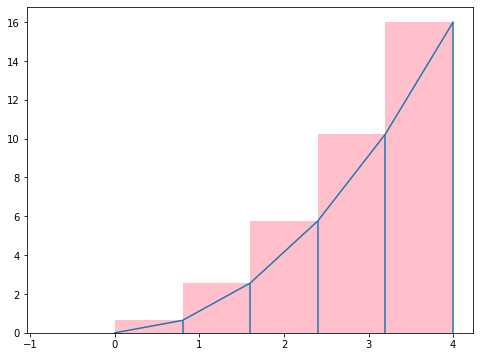
\includegraphics[width=0.8\textwidth]{./Imagens/Integral de Riemann/RI3.png} 
	\caption{Aproximação superior}
	\label{fig:RI3}
\end{figure}

A área da região S será tanto mais próxima do valor real $21.333$ quanto mais retângulos utilizarmos para dividir a área:

\begin{minted}{python}
import numpy as np

def area(a,b,n):
y = np.linspace(a,b,n+1)
w = (b - a)/n
f = lambda x: x**2
S = 0

for i in y[1:]:
	S = S + f(i)*w 
	
	print(f"Área: {S:.3f} (para {n} retângulos)")

area(0,4,5)
# Área: 28.160 (para 5 retângulos)
area(0,4,100)
# Área: 21.654 (para 100 retângulos)
area(0,4,500)
# Área: 21.397 (para 500 retângulos)
area(0,4,1000)
# Área: 21.365 (para 1000 retângulos)
area(0,4,5000)
# Área: 21.340 (para 5000 retângulos)
area(0,4,10000)
# Área: 21.337 (para 10000 retângulos)

\end{minted}

\subsection{Exemplo por aproximação inferior}

Vamos resolver a mesma integral de Riemann por aproximação inferior. Para isso, vamos dividir a área S em diversos retângulos de base $[x_{i-1},x_{i}]$ e altura $f(x_{i-1})$

\begin{minted}{python}
import matplotlib.pyplot as plt

fig, ax = plt.subplots(figsize =(8,6))

a = 0
b = 4
n = 5
x = np.linspace(a,b,n+1)

f = lambda x: x**2
vetor = []
for i in x:
	vetor.append(f(i))
	plt.vlines(i,0,f(i))

y = x**2
plt.plot(x,y)
plt.bar(x[:-1], vetor[:-1], align='edge', 
width=(b-a)/n, color='pink')
plt.show()
\end{minted}

\begin{figure}[H]
	\centering
	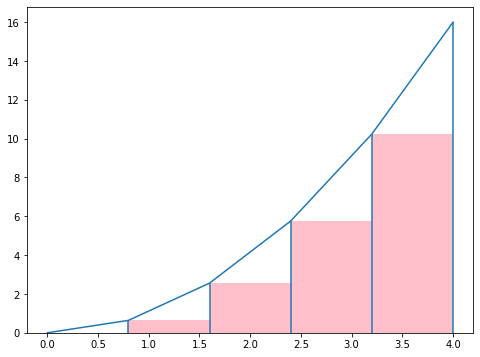
\includegraphics[width=0.8\textwidth]{./Imagens/Integral de Riemann/RI4.png} 
	\caption{Aproximação inferior}
	\label{fig:RI4}
\end{figure}

A área da região S será tanto mais próxima do valor real $21.333$ quanto mais retângulos utilizarmos para dividir a área:

\begin{minted}{python}
import numpy as np

def area(a,b,n):
y = np.linspace(a,b,n+1)
w = (b - a)/n
f = lambda x: x**2
S = 0

for i in y[:-1]:
	S = S + f(i)*w 

	print(f"Área: {S:.3f} (para {n} retângulos)")

area(0,4,5)
# Área: 15.360 (para 5 retângulos)
area(0,4,100)
# Área: 21.014 (para 100 retângulos)
area(0,4,500)
# Área: 21.269 (para 500 retângulos)
area(0,4,1000)
# Área: 21.301 (para 1000 retângulos)
area(0,4,5000)
# Área: 21.327 (para 5000 retângulos)
area(0,4,10000)
# Área: 21.330 (para 10000 retângulos)
\end{minted}

\subsection{Aplicações da Integral de Riemann}

\begin{itemize}
\item Pode ser utilizado na Matemática para: determinar a área de polígonos regulares ou irregulares; calcular a Transformada de Fourier; determinar o comprimento de uma curva; determinar o volume de um sólido.
\item Na física, é utilizado para: determinar a massa de um objeto caso a sua densidade seja conhecida; calcular o trabalho realizado partindo da força; calcular a velocidade e o instante dado a aceleração e as condições iniciais; calcular as equações de Maxwell.
\item Na engenharia é utilizado para determinar a força cortante e momento fletor; centroide de uma área; momento de inércia de uma área;
\item Na estatística é utilizado na função densidade de probabilidade.
\item Na química, pode ser utilizado para determinar a força a partir da pressão provocada por um conjunto de moléculas no interior de um recipiente.
\end{itemize}
   
\section{Oscilador Harmônico Amortecido}

\subsection{Conceitos}
O oscilador harmônico amortecido descreve o movimento mecânico de um oscilador (ex: pêndulo de massa-mola) sob a influência de uma força restauradora e atrito. O movimento do pêndulo depende basicamente de 3 forças:

\begin{itemize}	
\item Força de inércia $F = m \, \ddot{x}$
\item Força restauradora $F_{f} = -kx$
\item Força de amortecimento $F_{r} = -\mu \, \dot{x}$
\end{itemize}

\begin{figure}[H]
	\centering
	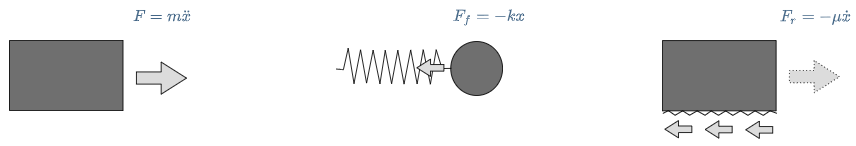
\includegraphics[width=0.8\textwidth]{./Imagens/Oscilador/OH1.png} 
	\caption{Tipos de forças atuantes}
	\label{fig:OH1}
\end{figure}

\subsection{Força de inércia}
Advém da 2° Lei de Newton que diz que a força resultante que atua sobre um corpo é igual ao produto de sua massa pela aceleração.

\subsection{Força restauradora}
É a força que puxa a massa do pêndulo de volta para sua posição de repouso. Esta força é diretamente proporcional ao deslocamento em relação à posição de equilíbrio.

\begin{itemize} 
\item $x$: é o deslocamento da posição de equilíbrio, em metros (m).
\item $k$: é a constante de proporcionalidade, dada por $\large \frac{mg}{L}$ e que depende do material.
\end{itemize}

\subsection{Força de amortecimento}
É a força de resistência ao movimento relativo entre superfícies sólidas, camadas de fluidos e outros materiais que deslizam um contra o outro. Essa força de atrito é proporcional à velocidade do pêndulo.
\begin{itemize}
\item $\dot{x}$:  velocidade de deslocamento de uma massa em relação a um ponto fixo.
\item $\mu$: é o coeficiente de atrito que depende do material e da forma da matéria
\end{itemize}

\subsection{Equação do movimento}

A força resultante será a soma da força restauradora e de amortecimento.

\[\large m \ddot{x} = -\mu \dot{x} -kx \rightarrow \ddot{x} + \frac{\mu}{m}\dot{x} + \frac{k}{m}x = 0\]
	
Esta equação é uma equação diferencial linear, homogênea, de segunda ordem e com coeficientes constantes. 

\begin{itemize}

\item Vamos definir $\large \omega _{0} = \sqrt{\frac{k}{m}}$ como a frequência natural de vibração não amortecida do sistema.

\item Vamos definir a sigla $\zeta$ como o \textbf{coeficiente de amortecimento} ou simplesmente \textbf{amortecimento}, sendo a sua fórmula:

\[ \large \zeta = \frac{\mu}{2\sqrt{km}} \]

\item Vamos considerar ainda $\large p = \frac{dx}{dt}$.

\end{itemize}

A equação do movimento, fica, então:

\[ \large \frac{dp}{dt} = -2\zeta w_{0} p - w_{0}^2x \]

O termo $-2\zeta w_{0}$ é responsável pelo amortecimento. Caso o coeficiente de amortecimento $-2\zeta w_{0}$ seja nulo, o sistema passa a oscilar indefinidamente, realizando um \textbf{Movimento Harmônico Simples (MHS)}.

\subsection{Amortecimento}

\begin{itemize}
	
\item O amortecimento é uma influência dentro ou sobre um sistema oscilatório que tem o efeito de reduzir, restringir ou prevenir suas oscilações.
 
\item O \textbf{coeficiente de amortecimento} é uma medida adimensional que descreve como as oscilações em um sistema decaem após uma perturbação. Muitos sistemas exibem comportamento oscilatório quando são perturbados de sua posição de equilíbrio estático.

\item Uma massa suspensa por uma mola pode, se puxada e liberada, pular para cima e para baixo. O sistema tende a retornar à sua posição de equilíbrio a cada salto, mas a ultrapassa. Às vezes, as perdas (por exemplo, atrito) amortecem o sistema e podem fazer com que as oscilações diminuam gradualmente em amplitude para zero ou se atenuem. O \textbf{coeficiente de amortecimento} é uma medida que descreve a rapidez com que as oscilações diminuem de um salto para o outro. 

\end{itemize}

\subsubsection{Fórmula do amortecimento}

O coeficiente de amortecimento é geralmente representado pela sigla $\zeta$ e sua fórmula é:

\[ \large \zeta = \frac{\mu}{2\sqrt{km}}\]

\subsubsection{Tipos de amortecimento}

O coeficiente de amortecimento ($\zeta$) fornece indicações de como será a resposta transitória do sistema:

\begin{itemize}
\item Se $\zeta > 1$: sistema superamortecido (overdamped). O sistema retorna (decai exponencialmente) para o estado estável sem oscilar.
\item Se $\zeta = 1$: sistema criticamente amortecido (critically damped). O sistema retorna para o estado estável rapidamente e sem oscilar.
\item Se $0 < \zeta < 1$: sistema subamortecido (underdamped).  O sistema oscila com uma freqüência levemente diferente que o do caso não amortecido com a amplitude gradualmente decrescendo a zero.
\item Se $\zeta = 0$: sistema não amortecido. O sistema oscila sem perda de amplitude.

\end{itemize}


\subsection{Oscilador harmônico amortecido no Python}

O gráfico da posição vs tempo de um oscilador harmônico foi obtido com o uso da biblioteca \textbf{odeint} do Python, que possibilita o usuário a encontrar as soluções de um sistema de equações diferenciais ordinárias.

\begin{minted}{python}
from scipy . integrate import odeint
import numpy as np
from matplotlib import pyplot as plt

def dy(y, t, zeta, w0):
x, p = y[0], y[1]
dx = p
dp = -2 * zeta * w0 * p - w0**2 * x
return [dx, dp]

# estado inicial
y0 = [1.0, 0.0]

# intervalo de tempo
t = np.linspace(0, 10, 1000)
w0 = 2*np.pi*1.0 # frequência natural
# print(w0)

# resolvendo a EDO para 4 diferentes 
# valores de amortecimento
# não amortecido
y1 = odeint(dy, y0, t, args=(0.0, w0)) 
# sub-amortecido
y2 = odeint(dy, y0, t, args=(0.2, w0))
# criticamente amortecido 
y3 = odeint(dy, y0, t, args=(1.0, w0)) 
# super-amortecido
y4 = odeint(dy, y0, t, args=(5.0, w0)) 

fig, ax = plt.subplots(figsize = (10,8))
ax.plot(t, y1[:,0], 'k', label="não amortecido", 
linewidth=0.5)
ax.plot(t, y2[:,0], 'r', label="sub-amortecido")
ax.plot(t, y3[:,0], 'b', label=r"criticamente amortecido")
ax.plot(t, y4[:,0], 'g', label="super-amortecido")
ax.legend()
plt.show()
\end{minted}

\begin{figure}[H]
	\centering
	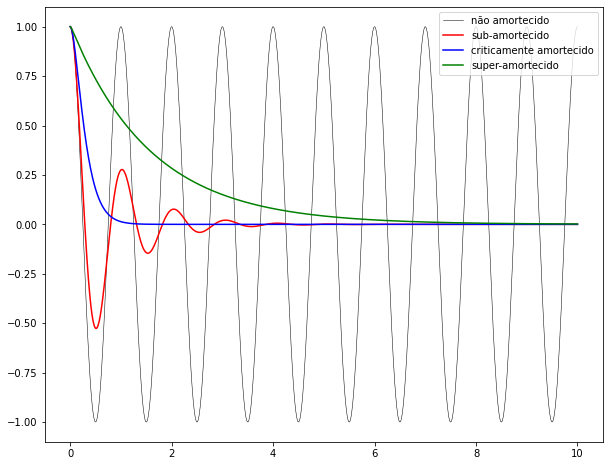
\includegraphics[width=0.8\textwidth]{./Imagens/Oscilador/OH2.png} 
	\caption{Gráfico posição x tempo}
	\label{fig:OH2}
\end{figure}

\subsection{Aplicações da oscilação harmônica amortecida}

\begin{itemize}
\item Em sistemas físicos, o amortecimento é produzido por processos que dissipam a energia armazenada na oscilação. Os exemplos incluem arrasto viscoso em sistemas mecânicos, resistência em osciladores eletrônicos e absorção e dispersão de luz em osciladores ópticos. 
\item Na engenharia elétrica, as repostas naturais de circuitos RLC podem ser super-amortecido, criticamente amortecido, sub-amortecido ou sem amortecimento.
\item Os amortecedores de um carro amortecem criticamente a suspensão do veículo e, portanto, resistem à vibrações que poderiam dificultar o controle ou causar danos. 
\item Amortecedores de porta evitam que a porta oscile quando ela é fechada graças à esse princípio.
\end{itemize}
\chapter{Conclusão}

\section{Conclusões}
... 

\section{Trabalhos futuros}
...
\section{Oscilador Harmônico Simples}

\subsection{Movimento Periódico}

Um movimento é dito periódico quando um objeto saí de uma posição e, após um certo intervalo de tempo chamado Período ($T$), retorna a essa posição original com a mesma velocidade. Matematicamente falando:

\begin{equation}
\large \vec{r}(t + T) = \vec{r}(t)
\tag{8.1}
\end{equation}

\begin{equation}
\large \vec{v}(t + T) = \vec{v}(t)
\tag{8.2}
\end{equation}

Onde $\vec{r}$ e $\vec{v}$ são respectivamente os vetores posição e velocidade deste objeto.  
Outra característica importante de um movimento periódico é a frequência ($f$) que representa o número de vezes que o movimento se repete em uma unidade de tempo. Tal propriedade é definida como sendo o inverso do Período:

\begin{equation}
\Large f = \frac{1}{T}
\tag{8.3}
\end{equation}


\subsection{Força elástica}

É a força que proporciona o movimento periódico. As vezes denominada força restauradora, esta tende a restaurar o equilíbrio retornando o objeto a posição de equilíbrio toda vez que o mesmo é deslocado. Esse tipo de força tem a forma semelhante a:

\begin{equation}
\large F = -kx
\tag{8.4}
\end{equation}

A variável $k$ representa a constante elástica da mola, e é especifica para o material que compõe a mola.

\subsection{Equação do movimento}

Pela segunda lei de newton, sabemos que a força resultante sobre um objeto é igual ao produto da massa pela aceleração deste.  Podemos determinar uma equação que descreva a posição de um objeto em função do tempo, a partir da segunda lei de newton. Imagine um corpo qualquer de massa $m$ preso a uma mola de constante elástica $k$, como na figura abaixo.

\begin{figure}[H]
	\centering
	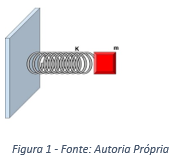
\includegraphics[width=0.5\textwidth]{./Imagens/OHS/ohs1.png} 
	\caption{Sistema massa-mola}
	\label{fig:OHS1}
\end{figure}

Considerando que a força aplicada a esse corpo de massa $m$, seja a força restauradora mencionada acima, temos que:

\begin{equation}
\Large ma = -kx
\tag{8.5}
\end{equation}

Podemos escrever a aceleração $a$ como sendo a segunda derivada em relação ao tempo t. Sendo assim, a equação acima fica: 

\begin{equation}
\Large m \frac{d^2x(t)}{dt^2} = -kx(t)
\tag{8.6}
\end{equation}


Temos em mãos, então, uma equação diferencial ordinária (EDO) que delimita a posição de um oscilador harmônico simples (OHS) em função do tempo.

Para determinarmos a expressão da função $x(t)$, precisamos resolver essa equação acima.  O intuito do presente trabalho é utilizar computação numérica, com a linguagem Scilab para isso. 

Antes de tudo é necessário utilizar um artificio matemático para transformar a EDO de 2ª ordem acima, em um sistema de 2 EDO’s de 1ª ordem. Para isso, fazemos: 

\[\Large \frac{dx(t)}{dt} = v\]

Dessa forma, fica implícito que:

\[\Large \frac{dv}{dt} = \frac{d^2x(t)}{dt^2}\]

Portanto, fazendo as devidas substituições temos o seguinte sistema:

\begin{equation}
\Large \frac{dx(t)}{dt} = v
\tag{8.7}
\end{equation}

\begin{equation}
\Large \frac{dv}{dt} = -\frac{k}{m}x(t)
\tag{8.8}
\end{equation}

Com isso aplicamos o método numérico de Euler para o sistema acima:

\begin{minted}{Scilab}
//Resolução da equação de movimento para OHS
//A equação é: X''(t) = -(k/m)X(t) uma edo de 2ª ordem

//Parâmetros do problema
//m = 1kg; K = 1N/m; 
//Intervalo de tempo  = 0 à 40 segundos 
// deslocamento da mola incialmente é 0.20 metros
// velocidade no instante t = 0 é 0 metros/segundo

clear,clc
// definindo o intervalo de tempo
t0 = input("informe o valor inicial do intervalo: ");
tn = input("informe o valor final do intervalo: ");
h = input("Informe o passo h: ");
t = t0:h:tn // criando o vetor intervalo de tempo
t = t' // apenas transpoe o vetor t
k = input("informe a constante da mola:")
m = input("informe a massa do objeto: ")

//condições iniciais
// objeto deslocado 0.20 m da posição de equilibrio
w1(1) = 0.20 
// no instante que o objeto é solto, 
// têm se velocidade igual a zero
w2(1) = 0 

for j = 2:length(t)
w1(j) = w1(j-1) + w2(j-1)*h //diz respeito a X(t)
w2(j) = w2(j-1) -(k/m)*w1(j-1)*h // diz respeito a V(t)
end
// determinado para o caso especifico 
// de m = 1kg, k = 1N/m, X(0) = 0.20m, theta_inicial  = 0
function x = f(t)
//w1(1) corresponde ao deslocamento inicial da mola
x = w1(1)*cos(sqrt(k/m)*t) 
endfunction
plot2d(t,[w1, f()], leg = "Numérico@Exata@")
\end{minted}
\section{Pêndulo Simples}

O pêndulo simples é um sistema teórico composto por uma esfera de massa $m$ suportada por uma corda fina ou fio de massa desprezível. Tal sistema é um exemplo de um movimento harmônico simples.

O movimento de um pêndulo oscilante é estudado fazendo se as devidas considerações que simplificam essa análise.

\begin{figure}[H]
	\centering
	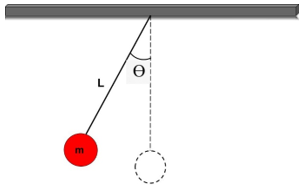
\includegraphics[width=0.8\textwidth]{./Imagens/Pendulo simples/ps1.png} 
	\caption{Sistema pêndulo simples}
	\label{fig:PS1}
\end{figure}

Este movimento pode ser descrito pela seguinte expressão:

$$\Large \frac{d^2\theta}{dt^2} + \frac{g}{L}sen(\theta) = 0$$

Onde $\theta$ representa o ângulo de deslocamento da esfera em relação a posição de equilíbrio na vertical, $t$  o tempo, $g$ a aceleração da gravidade e $L$ o comprimento do fio.

Temos aqui uma equação diferencial ordinária de 2ª ordem de resolução analítica relativamente complexa.

Para simplificação da resolução é feita a seguinte aproximação: para ângulos pequenos ($\theta \ll 1$),  $sen(\theta)  \approx  \theta$.  A equação se torna então: 

$$\Large \frac{d^2\theta}{dt^2} + \frac{g}{L}\theta = 0$$

Entretanto tem – se um desvio considerado do comportamento real desse sistema aplicando – se essa simplificação. Para contornar isso, podemos recorrer a métodos numéricos que fornecem com precisão satisfatória a resolução da equação original (sem a simplificação) supracitada.

Para isso vamos utilizar o software Scilab e sua linguagem para resolver essa EDO de 2ª ordem. Aplicaremos o método de Euler que consiste em um dos métodos de passo único no que tange a resolução de equações diferenciais ordinárias. Antes de tudo temos que transformar essa equação de 2ª ordem em um sistema com duas equações de 1ª ordem. Chamamos a $\large \frac{d\theta(t)}{dt} = \omega$, assim, por consequência temos que a derivada segunda de $\theta$ é igual a $\large \frac{d^2\theta}{dt^2} = \frac{d\omega}{dt}$ sendo assim podemos substituir tais termos na equação 4, resultando no seguinte sistema:

$$\Large \frac{d\theta(t)}{dt} = \omega$$

$$\Large \frac{d\omega}{dt} = -\frac{g}{L} sen(\theta(t))$$

Sendo assim, aplicamos o método de Euler no sistema para determinar o comportamento de $\theta(t)$ em relação ao tempo:

\begin{minted}{Scilab}
// resolução de sistema de 2 equações representando 
// o movimento de um pêndulo simples
clear,clc
// definindo o intervalo de tempo
t0 = input("informe o valor inicial do intervalo: ");
tn = input("informe o valor final do intervalo: ");
h = input("Informe o passo h: ");
t = t0:h:tn // criando o vetor intervalo de tempo
t = t' // apenas transpoe o vetor t

L = input("informe o comprimento do fio")
g= 9.8 //aceleração da gravidade

//condições iniciais
w1(1) = 0.785398163 // 45 graus em radianos
w2(1) = 0
for j = 2:length(t)
w1(j) = w1(j-1) + w2(j-1)*h
w2(j) = w2(j-1) -(g/L)*sin(w1(j-1))*h
end

//solução linear 
function y = f(t)
y = 0.785398163*cos(sqrt(g/L)*t)
endfunction

plot(t,w2,'b', t, f, 'r')
legends(["Não Linear", "Linear"], opt = "lr")
\end{minted}
\section{Método da bissecção}

\subsection{Encontrando raízes de equação - Caso do paraquedista}

A raiz de uma $f(x)$ é um valor de $x$ (variável independente) que ao ser substituído na expressão da função, o valor desta se iguala a zero, em outras palavras:

\begin{equation}
\Large f(x) = 0
\tag{10.1}
\end{equation}

Apesar muitas funções possuírem modos analíticos de encontrar suas raízes, uma parcela considerada de outras funções não contêm tal facilidade. Nesse caso são necessários métodos numéricos para determinar tais valores. Existem vários métodos para determinar as raízes de uma equação, como os métodos intervalares, os métodos abertos, entre outros.

\subsection{Motivação}

Imagine uma função ($v$) que mede a velocidade de um paraquedista de massa m caindo sob a força da aceleração da gravidade:

\begin{equation}
\Large v = \frac{gm}{c}(1-e^{(-\frac{c}{m})t})
\tag{10.2}
\end{equation}

Sendo $c$ o coeficiente de arrasto e $t$ o tempo em questão. De posse dos valores da massa do paraquedista e do coeficiente de arrasto, é fácil resolver analiticamente essa equação para determinar o valor de $t$ que zera a função, pois $v$ é expressa explicitamente na equação.

Entretanto, se o objetivo fosse determinar o coeficiente de arrasto para que um paraquedista de uma certa massa $m$ atinja uma certa velocidade $v$ num determinado intervalo de tempo, perceberia – se que isso não seria possível, pois não há como isolar a variável $c$ em um dos lados da equação. Dizemos então que $c$  está implícito na equação.

Esse mesmo tipo de problema ocorre com frequência na área da engenharia, e para a resolução destes utilizam – se os métodos numéricos de raízes de equações. Abordaremos um destes, o método da bissecção, logo a seguir.

\subsection{Método da bissecção}

O método da bissecção se encaixa no grupo dos métodos intervalares que se baseiam numa consequência do Teorema do Valor Intermediário:

Se o valor de um função f(x) muda de sinal em algum ponto do intervalo [a,b], em outras palavras:

\begin{equation}
\Large f(a) \cdot f(b)<0
\tag{10.3}
\end{equation}

Obrigatoriamente deve existir pelo menos um valor $\varepsilon$ pertencente a esse intervalo [a,b] que é raiz dessa função.

\begin{figure}[H]
	\centering
	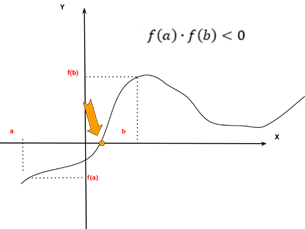
\includegraphics[width=0.5\textwidth]{./Imagens/Bissec/bi1.png} 
	\caption{Teorema do valor intermediário}
	\label{fig:OHS1}
\end{figure}

Os métodos de busca incrementais tiram vantagem dessa observação localizando um intervalo no qual a função muda de sinal. Então, a posição da mudança de sinal (e, consequentemente, da raiz) é identificada mais precisamente, dividindo-se o intervalo em diversos subintervalos. Procura-se em cada um desses subintervalos para localizar a mudança de sinal. O processo é repetido e a estimativa da raiz é refinada dividindo-se os subintervalos em incrementos menores.

Na prática, não temos o valor da raiz exata, afinal esse é o intuito do método, e por isso utiliza – se um critério de parada que é o erro em relação ao valor da raiz anteriormente calculado. Como o intervalo diminuí a cada iteração, podemos preestabelecer um valor de erro aceitável para encontrar um valor aproximado da raiz exata.

Podemos utilizar o método acima para resolver o problema do paraquedista mencionado anteriormente.  Para isso, precisamos rearranjar a equação (14) subtraindo $v$ de ambos os lados. Chamamos, então, essa função de $f(c)$:

\begin{equation}
\Large f(c) = \frac{gm}{c}(1-e^{(-\frac{c}{m})t}) - v
\tag{10.4}
\end{equation}

Imaginando um paraquedista de 68.1 kg caindo a uma velocidade de 40 m/s no tempo t = 10s e adotando a aceleração da gravidade como 9.81m/s², temos que a equação passa a ser:

$$\Large f(c) = \frac{668,06}{c}(1 - e^{-0.146843c})-40$$

\begin{minted}{Scilab}
// Algoritmo para encontrar raízes 
// de um função utilizadndo o método da bissecção 
// Escreva aqui a função de uma variável 
function y = f(x); 
y = (668.06/x)*(1-exp(-0.146843*x)) - 40 
endfunction

function acha_raiz(lim_inf, lim_sup, erro) 
//encontra a raiz aproximada de uma função, 
//quando fornecido o limite inferior, 
//o superior e o erro aceitável    
	while (1)
		raiz = (lim_inf + lim_sup)/2
//caso o intervalor encontrado seja menor 
//que o erro informado, achamos a raiz
		if abs(lim_sup - lim_inf) < erro then
			printf("Raiz aproximada encontrada:")
			x = (lim_inf+lim_sup)/2
			break;
// se esse produto é positivo, 
// significa que a raiz está no intervalor superior
		elseif f(lim_inf)*f(raiz) > 0 then 
			lim_inf = raiz;
// se as duas possibilidades acima não estão corretas, 
// só resta que a raiz está no intervalo inferior
		elseif f(lim_inf)*f(raiz) < 0  
			lim_sup = raiz                
		end
	end
// Observe que o intervalo vai sempre sendo diminuído
	disp(x);
printf("Valor da função aplicada na raiz 
aproximada encontrada:\ny = ")
	disp(f(x))

endfunction

x = linspace(-20,20,50)
plot(x,f)
\end{minted}

\begin{minted}{Scilab}
while(1)
a = input("Informe o limite inferior do intervalo: ");
b = input("Informe o limite superior do intervalo: ");
erro = input("Informe o erro/Críterio De Parada desejado: ")

// verifica se raiz se encontra entre o intervalo fornecido
if f(a)*f(b) < 0 then 
printf("O intervalo possui uma ou mais raizes\n")
// caso a raiz esteja aqui, 
//ele interrompe o loop e vai pra frente no algoritmo
break 
else
printf("Esse intervalo não possue raiz, insira um novo!")
end
end
acha_raiz(a,b,erro);
\end{minted}

Como visto no código, a raiz aproximada encontrada foi de $c = 14.801636$, se substituirmos na equação original para calcular a velocidade, verificaremos que o valor (39.999035) se aproxima de $40 m/s$ como estipulado.
\section{Idealidade dos gases}
	
\subsection{Determinação das constantes a e b na equação de Van Der Walls}

A equação dos gases ideais determina o comportamento de gases considerados ideais. O gás ideal é um modelo teórico, que se considera nula a interação entre as moléculas do gás. A equação é definida como:

\begin{equation}
\Large PV=nRT
\tag{11.1}
\end{equation}

Onde $P$ é a pressão absoluta,  $V$ é o volume do gás,  $n$ é o número de moles, $R$ constante universal dos gases e $T$ é a temperatura que o gás se encontra. 

Na prática sabe – se que as interações entre as moléculas de um gás são consideráveis, mas existem intervalos de pressão e temperatura em que alguns gases se aproximam do comportamento de um gás ideal (uns mais que outros) e essa equação é válida.

Uma equação alternativa a equação dos gases ideais é a equação de Van der Waals proposta por J.D. van der Waals em 1873:

\begin{equation}
\Large (P + \frac{a}{v^{2}} )(v-b)=RT
\tag{11.2}
\end{equation}

Nesse modelo proposto, $a$ e $b$ são constantes empíricas e $v$ é o volume molar do gás $(\large v=\frac{V}{n})$. A constante $a$ representa a intensidade das interações atrativas entre as partículas do gás e $b$ representa a intensidade das interações repulsivas. Essas constantes são características de cada gás e independem da temperatura.

Em projetos de engenharia envolvendo gases é, frequentemente, necessário determinar o volume que determinado número de moles de um gás ocupa a uma determinada pressão e temperatura. 
Vamos determinar o volume molar dos gases $N_{2}$ e $NH_{3}$ e comparar com o volume de um gás ideal calculado a partir da equação do gás ideal.

\begin{minted}{Scilab}
function raiz(xo, erro, iter_max, a, b, temp, P)  

// escreva aqui a equação que vc deseja determinar a raiz
function W = f(x) 
W = (P + a/(x^2))*(x - b) - 0.082054*temp
endfunction
// informe aqui a derivada da (função acima)
// em relação a varíavel dependente acima
function deriv = f_linha(x) 
deriv = P - (a/x^2) + (2*a*b)/x^3
endfunction
i = 1
X(i) = xo
// Quando o erro relativo for menor que
// o erro fornecido pelo usuário o loop é quebrado
while (2>1) 
// equação de Newton Raphson
X(i+1) = X(i) - (f(X(i))/f_linha(X(i))) 
if abs((X(i+1) - X(i))/X(i+1)) < erro
break
elseif i > iter_max
break
end
i = i+1
end   
printf("volume molar do gás com a equação de van der waals:")
disp(X(i))   
endfunction
// calcula o volume molar do gás ideal
function gas_ideal(P, T)
// 0.082054 é a constante universal dos gases R
vol = (0.082054*T)/P 
printf("Volume molar considerando gás como ideal:")
disp(vol)
endfunction 
\end{minted}

\begin{figure}[H]
	\centering
	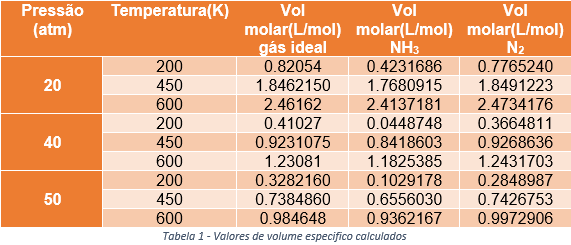
\includegraphics[width=0.8\textwidth]{./Imagens/Idealidade/ide1.png}
	\caption{Tabela dos gases}
	\label{fig:OHS1}
\end{figure}
\section{Integração Numérica - Quantidade de calor}

Nas engenharias e nas ciências, frequentemente se quer determinar o quanto de calor precisa ser fornecido, a uma determinada substância, para que esta saia de uma temperatura inicial para uma temperatura final. Para isso é necessário determinar a capacidade calorifica do material em questão. A fórmula abaixo mostra o cálculo da quantidade de calor utilizando a capacidade calorífica:

\begin{equation}
\Large Q = mc \Delta T
\tag{12.1}
\end{equation}

\begin{itemize}
\item Onde $Q$ é a quantidade de calor, $m$ a massa em questão,  $c$ a capacidade calorífica e delta $\Delta T$ a variação de temperatura desejada.
\item $c$ diz respeito a quantidade de energia necessária que deve ser fornecida (ou retirada do) ao material para que uma unidade de massa desse material varia sua temperatura em uma unidade de temperatura.
\end{itemize}

A capacidade calorífica é definida de duas formas, capacidade calorífica a volume constante $C_{V}$ e a capacidade calorifica a pressão constante, $C_{P}$.

Entretanto, um problema prático surge. A capacidade calorífica é constante (não depende da temperatura) para pequenos intervalos de temperatura, mas para intervalos maiores $c$ já não é mais constante e passa a variar com a temperatura sob a forma da seguinte equação empírica:

\begin{equation}
\Large \frac{C_{P}}{R} = A + BT + CT^2+DT^{-2}
\tag{12.2}
\end{equation}

Os parâmetros $A$ , $B$, $C$ e $D$ são independentes da temperatura, mas acabem por sofrer influência do valor da pressão constante. Normalmente, os dois últimos parâmetros são iguais a zero para uma grande gama de substâncias.

Visto que a fração do lado esquerdo da equação acima é adimensional, as unidades de  $C_{P}$ são as escolhidas para a constante universal dos gases $R$.

Vamos determinar a a quantidade de calor necessária para elevar a temperatura da amônia de 10°C à 100°C utilizando integração numérica no Python.

Existe uma biblioteca da linguagem Python chamada Scipy voltada para ciências e engenharias que possui o pacote de integração \textbf{scipy.integrate}. Nesse pacote utilizaremos a função \textbf{quad} que recebe como parâmetros a função a ser integrada, e o intervalo de integração delimitados pelo valor inicial $a$ e o valor final $b$. Essa função retorna ainda, o valor numérico da integração e o uma estimativa do erro numérico associado ao método de integração utilizado.

Os valores dos parâmetros $A$, $B$, $C$ e $D$ para Amônia são retirados do livro Introdução à Termodinâmica da Engenhara Química (SMITH, J.M. et al), mais especificamente na tabela C.3 do apêndice C.

$$\Large A=22,626; B=-100,75.10^{-3}; C = 192,71.10^{-6}$$

Sendo assim, temos que buscamos integrar a seguinte expressão:

\begin{equation}
\Large \Delta H = \int_{283K}^{373K} \frac{C_{p}}{R}dt
\tag{12.3}
\end{equation}

$$\Large \Delta H = \int_{283K}^{373K} (22,626 - 100,75.10^{-3}T + 192,71.10^{-6}T^2)dT$$

\begin{minted}{Scilab}
from scipy.integrate import quad
#importa a função quad para integrar numericamente uma função

#definindo a função em questão para utilizar 
#na função quad
def funcao(T):
#função de Cp para a amônia 
return 22.626 - 0.10075*T + 0.00019271*(T**2) 

# 10 °C e 100°C na escala Kelvin respectivamente
c, erro = quad(funcao, 283, 373) 

print("o resultado é: {:f} (+-{:g})"
# é necessário multplicar o resultado 
# pelo valor da Constante universal dos gases R = 8.413
.format(c*8.314, erro)) 
\end{minted}
\section{Sistema de equações lineares – concentração de reatores}

Sistema de equações são vistos com frequência em problemas que envolvem a engenharia química. Com o princípio de conservação das massas, vários problemas são modelados utilizando essas entidades matemáticas. Talvez o exemplo mais famoso é o que envolve vários reatores ligados entre si. O princípio de conservação de massas resulta em balanços efetuados em um “recipiente” (no caso um reator) expressos matematicamente por:

\begin{center}
	Acumulação = Entrada – Saídas
\end{center}

\begin{figure}[H]
	\centering
	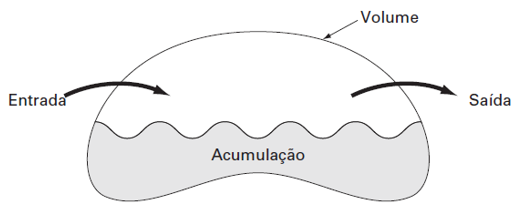
\includegraphics[width=0.8\textwidth]{./Imagens/Sistema de eq/sis1.png}
	\caption{Conservação da massa}
	\label{fig:sis1}
\end{figure}

Caso as entradas sejam maiores que saídas, têm – se um aumento da massa no interior, caso contrário, as saídas sejam maiores que as entradas, a massa no interior diminui. Chamamos de estado estacionário, ou regime permanente, quando o somatório das entradas se iguala ao somatório das saídas. Dessa forma o acúmulo é zerado e sobra:

\begin{center}
Entrada = Saídas
\end{center}

Imagine a seguinte situação. 5 reatores em série conectados entre sim, nos quais a alimentação de um ou mais reatores é a saída de um ou mais reatores, como mostra a imagem a seguir:

\begin{figure}[H]
	\centering
	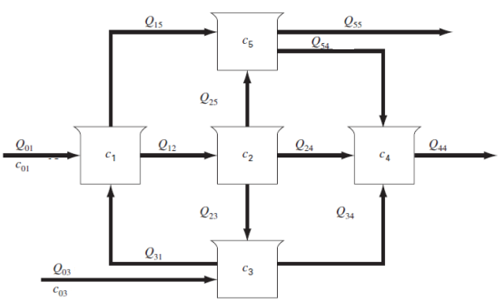
\includegraphics[width=0.8\textwidth]{./Imagens/Sistema de eq/sis2.png}
	\caption{Esquema de reatores}
	\label{fig:sis2}
\end{figure}

Na qual $Q_{ij}$ (vazão) representa a saída do reator $i$ alimentando o reator $j$. Por exemplo, $Q_{24}$ informa que uma das saídas do reator 2 alimenta o reator 4. As concentrações de cada reator são denotadas pelos $c_{i}$ ($i = 1, 2, ..., 5$). A taxa de massa que sai (ou entra) em cada reator é calculada multiplicando a vazão, dada em  $\large \frac{m^3}{min}$ , com a concentração dada em $\large \frac{mg}{m^3}$. 

Para o reator 1, há duas entradas e duas saídas como indicam as setas na figura acima, então o balanço de massa fica:

\begin{equation}
\large Q_{01} c_{01}  + Q_{31} c_{3}  = Q_{15} c_{1}+ Q_{12} c_{1}
\tag{13.1}
\end{equation}

Vamos aplicar método numérico para resolver situação – problema semelhante da figura acima, onde os valores das vazões são fornecidos, como as concentrações que alimentam os reatores 1 e 3. O objetivo é determinar as concentrações dos 5 reatores ($c1, c2, c3, c4, c5$). 
As razões fornecidas são: 

$$
\large Q_{01} = 5, Q_{31} = 3, Q_{25} = 2, Q_{23} = 2
$$

$$
\large Q_{15} = 4, Q_{55} = 3, Q_{54} = 3, Q_{34} = 7
$$

$$
\large Q_{12} = 4, Q_{03} = 8, Q_{24} = 0, Q_{44} = 10, c_{01} = 10, c_{03} = 20
$$

Repetindo o procedimento acima, para os 5 reatores, temos o seguinte sistema:

$$\large 8c_{1}  - 3c_{3}  = 50$$

$$\large 4c_{1}  - 4c_{2}  = 0$$

$$\large 10c_{3}  - 2c_{2}  = 160$$

$$\large -7c_{3} + 10c_{4} - 3c_{5}  = 0$$

$$\large 4c_{1}  +2c_{2}  -6c_{5}  = 0$$

O sistema acima pode ser reescrito na forma de multiplicação matricial, do tipo:

\begin{equation}
\large Ax + b = 0
\tag{13.2}
\end{equation}

Onde $A$, no nosso caso, representa a matriz 5x5 dos coeficientes do sistema
acima, $x$ é o vetor coluna 5x1 com os valores das concentrações que queremos determinar, por último, $b$ é vetor coluna dos componentes independentes.

$$\large A = \begin{bmatrix} 8 & 0 & -3 & 0 & 0 \\ 4 & -4 & 0 & 0 & 0 \\ 0 & -2 & 10 & 0 & 0 \\ 0 & 0 & -7 & 10 & -3 \\ 4 & 2 & 0 & 0 & -6 \end{bmatrix}$$

$$\large b = \begin{bmatrix} -50 \\ 0 \\ -160 \\ 0 \\ 0 \end{bmatrix}$$

$$\large x = \begin{bmatrix} C_{1} \\ C_{2} \\ C_{3} \\ C_{4} \\ C_{5} \end{bmatrix}$$

Utilizando o \textbf{Linsolve}, função embutida para o Scilab, podemos resolver o sistema acima e encontrar os valores das concentrações. A função linsolve calcula todas as soluções para problemas do tipo $\large Ax + b = 0$.

\begin{minted}{Scilab}
// sistema de equações algébricas lineares
// utilizaremos a função Linsolve para 
// resolver um sistema simulando a 5 reatores ligados entre si
// Queremos determinar as concetrações 
// c1, c2, c3, c4, c5 (referente a cada reator)

clear, clc

//informe aqui a seu sistema do tipo Ax + b = 0
A = [8 0 -3 0 0;4 -4 0 0 0;0 -2 10 0 0; 0 0 -7 10 -3;4 2 0 0 -6] 
// matriz dos coeficientes
b = [-50; 0; -160; 0; 0] 
x = linsolve(A, b)

printf("O vetor x é: \n")
mprintf("C1 = %6.4f \n", x(1))
mprintf("C2 = %6.4f \n", x(2))
mprintf("C3 = %6.4f \n", x(3))
mprintf("C4 = %6.4f \n", x(4))
mprintf("C5 = %6.4f \n", x(5))
\end{minted}
\chapter{Conclusão}

\section{Conclusões}
A partir do desenvolvimento de exemplos que abrangem as mais diversas áreas da ciência e engenharia utilizando a linguagem Python e Scilab, percebeu-se o quão prático é o uso dessa ferramenta no ensino e apresentação visual dos conceitos fundamentais. A disponibilidade de uma extensa gama de bibliotecas que possibilita a sua aplicação em diversos ramos do conhecimento mostrou que o uso dessas ferramentas é bastante conveniente na elaboração de materiais educacionais. 

\section{Trabalhos futuros}
Espera-se para os trabalhos futuros um aumento gradativo na complexidade das áreas de atuação do projeto, utilizando-se como referência as bases descritas e exemplificadas nesse projeto. %Conclusoes e trabalhos futuros
\chapter{REFERÊNCIAS}

Matthes, Eric. \textbf{Python Crash Course: A Hands-On, Project-Based Introduction to Programming}. 2 ed. 2019.

Halliday, David. \textbf{Fundamentos de Física. Eletromagnetismo - Volume 3}. LTC. 10 ed. 2016.

Moran, Michael J.; Shapiro, Howard. \textbf{Fundamentals of Engineering Thermodynamics}. 8 ed. 2014.

Géron, Aurélien. \textbf{Hands on Machine Learning with Scikit Learn Keras and TensorFlow}. O’Reilly Media. 2 ed. 2019. 

Stewart, James. \textbf{Cálculo - Volume 1}. Cengage Learning Nacional. 7 ed. 2014.






%---------- Referencias ----------
\clearpage % this is need for add +1 to pageref of bibstart used in 'ficha catalografica'.

\label{bibstart}
\bibliography{reflatex} % geracao automatica das referencias a partir do arquivo reflatex.bib
\label{bibend}

% %---------- Apendices (opcionais) ----------
% \apendice
% \chapter{Nome do Ap\^endice}

% Use o comando {\ttfamily \textbackslash apendice} e depois comandos {\ttfamily \textbackslash chapter\{\}}
% para gerar t\'itulos de ap\^en-dices.


% % ---------- Anexos (opcionais) ----------
%\anexo
%\chapter{Nome do Anexo}

% Use o comando {\ttfamily \textbackslash anexo} e depois comandos {\ttfamily \textbackslash chapter\{\}}
% para gerar t\'itulos de anexos.


% --------- Ordenacao Afabetica da Lista de siglas --------
%\textbf{* Observações:} a ordenacao alfabetica da lista de siglas ainda nao eh realizada de forma automatica, porem
% eh possivel se de realizar isto manualmente. Duas formas:
%
% ** Primeira forma)
%    A ordenacao eh feita com o auxilio do comando 'sort', disponivel em qualquer
% sistema Linux e UNIX, e tambem em sistemas Windows se instalado o coreutils (http://gnuwin32.sourceforge.net/packages/coreutils.htm)
% comandos para compilar e ordenar, supondo que seu arquivo se chame 'dissertacao.tex':
%
%      $ latex dissertacao
%      $ bibtex dissertacao && latex dissertacao
%      $ latex dissertacao
%      $ sort dissertacao.lsg > dissertacao.lsg.tmp
%      $ mv dissertacao.lsg.tmp dissertacao.lsg
%      $ latex dissertacao
%      $ dvipdf dissertacao.dvi
%
%
% ** Segunda forma)
%\textbf{Sugest\~ao:} crie outro arquivo .tex para siglas e utilize o comando \sigla{sigla}{descri\c{c}\~ao}.
%Para incluir este arquivo no final do arquivo, utilize o comando \input{arquivo.tex}.
%Assim, Todas as siglas serao geradas na ultima pagina. Entao, devera excluir a ultima pagina da versao final do arquivo
% PDF do seu documento.


%-------- Citacoes ---------
% - Utilize o comando \citeonline{...} para citacoes com o seguinte formato: Autor et al. (2011).
% Este tipo de formato eh utilizado no comeco do paragrafo. P.ex.: \citeonline{autor2011}

% - Utilize o comando \cite{...} para citacoeses no meio ou final do paragrafo. P.ex.: \cite{autor2011}



%-------- Titulos com nomes cientificos (titulo, capitulos e secoes) ----------
% Regra para escrita de nomes cientificos:
% Os nomes devem ser escritos em italico, 
%a primeira letra do primeiro nome deve ser em maiusculo e o restante em minusculo (inclusive a primeira letra do segundo nome).
% VEJA os exemplos abaixo.
% 
% 1) voce nao quer que a secao fique com uppercase (caixa alta) automaticamente:
%\section[nouppercase]{\MakeUppercase{Estudo dos efeitos da radiacao ultravioleta C e TFD em celulas de} {\textit{Saccharomyces boulardii}}
%
% 2) por padrao os cases (maiusculas/minuscula) sao ajustados automaticamente, voce nao precisa usar makeuppercase e afins.
% \section{Introducao} % a introducao sera posta no texto como INTRODUCAO, automaticamente, como a norma indica.

%\balance
\end{document}
